Optical flow \footnote{Optical flow,shorturl.at/mrtEZ}  คือรูปแบบของการเคลื่อนที่ของวัตถุในรูปภาพระหว่างภาพซึ่งอาจจะการจากเคลื่อน ที่ของวัตถุหรือตัวกล้อง ออกมาในรูปแบบของ เวกเตอร์(vector) 2 มิติ โดยที่เวกเตอร์แต่ละตัวจะแสดงถึงทิศทางการเคลื่อนที่ระหว่างภาพดังรูปด้านล่าง

\begin{figure}[!ht]
	\centering
	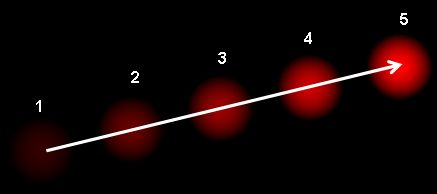
\includegraphics[width=1\textwidth]{chapter2/images/vector_optical.png}
		\caption{ตัวอย่างการเคลื่อนที่ของลูกบอล}
    	\label{fig:vector_optical}
\end{figure}

จากรูปภาพจะแสดงให้เห็นถึงการเคลื่อนที่ของลูกบอลของภาพที่ต่อเนื่องกัน 5 ภาพโดยที่ลูกศรแสดงถึงทิศทางการเคลื่อนที่ของเวกเตอร์
\\
\par
การทำงานของ optical flow อยู่บนสมมติฐานหลายประการได้แก่
\begin{enumerate}
	\setlength\itemsep{-0.25em}
	\item ความเข้มของพิกเซล(pixel) ของวัตถุจะไม่เปลี่ยนแปลงระหว่างภาพที่ต่อเนื่องกัน
	\item พิกเซลที่อยู่ใกล้กันจะมีการเคลื่อนไหวที่คล้ายกัน
\end{enumerate}

เมื่อพิจารณาพิกเซล I(x,y,t) จากภาพแรกจะเคลื่อนไหวเป็นระยะทาง (dx,dy) ไปยังภาพต่อไปหลังจากผ่านไปแล้ว dt เวลา ดังนั้นเนื่องจาก พิกเซล เหล่านี้เหมือนกันและความเข้มไม่มีการเปลี่ยนแปลง จึงทำให้พูดได้ว่า
\\
\begin{equation}
I(x,y,t) = I(x + dx, y + dy, t + dt)
\end{equation}
โดยที่
\begin{conditions}
I 		&	พิกเซลจากภายในภาพ				\\
x 		&	ตำแหน่งของพิกเซล ในแกน x 		\\
dx		&	ระยะทางที่เคลื่อนที่ในแกน x 			\\
y		&	ตำแหน่งของพิกเซล ในแกน y 		\\
dy		&	ระยะทางที่เคลื่อนที่ในแกน y 			\\
t 		&	เวลา							\\
dt		&	ระยะเวลาที่เปลี่ยนไประหว่างภาพ
\end{conditions}

จากนั้นใช้การประมาณค่าของ taylor series ทางฝั่งขวามือและ ลบค่า common term และหารด้วย dt เพื่อให้ได้สมการดังต่อไปนี้
\begin{equation}
f_{x}u + f_{y}v + f_{t}
\end{equation}
\begin{equation}
f_{x} = \frac{\delta f}{\delta x} ; f_{y} = \frac{\delta f}{\delta y}
\end{equation}
\begin{equation}
u = \frac{\delta x}{\delta t} ; v = \frac{\delta y}{\delta t}
\end{equation}
โดยที่
\begin{conditions}
f_{x}		&	เกรเดียน(gradient) ในแกน x 		\\
f_{y}		&	เกรเดียนในแกน y				\\
f_{t}		&	เกรเดียนของเวลา				\\
u 		&	เวกเตอร์การเคลื่อนที่ของแกน x 	\\
v		&	เวกเตอร์การเคลื่อนที่ของแกน y	\\
\end{conditions}
สมการข้างบนนี้จะเรียกว่าสมการ optical flow จากสมการทำให้สามารถหา $f_{x}$ และ $f_{y}$ โดยเป็น เกรเดียนของภาพ และ  $f_{t}$ เป็นเกรเดียน(gradient)ของเวลา แต่ $u$ กับ $v$ เป็นตัวแปรที่ไม่ทราบ ทำให้สมการนี้ไม่สามารถแก้ไขโดยมีตัวแปรที่ไม่ทราบถึง 2 ตัว จึงมีการนำวิธีการต่าง ๆ เข้ามาใช้ในการแก้ปัญหานี้ โดยวิธีการที่นำเข้ามาใช้ในการแก้ปัญหาคือ dense optical flow ซึ่งใช้อัลกอริทึมของ Gunner Farneback ซึ่งจะใช้วิธีการขยายพหุนาม\footnote{polynomial expansionfile:http://www.diva-portal.org/smash/get/diva2:273847/FULLTEXT01.pdf} (polynomial expansion)

